94. $\cfrac{3x^2+6x+2}{x^2+2x}+\cfrac{2x+2}{x-1}\geqslant\cfrac{5x+1}{x}
\Leftrightarrow 3+\cfrac{2}{x^2+2x}+2+\cfrac{4}{x-1}\geqslant 5+\cfrac{1}{x}
\Leftrightarrow \cfrac{2}{x(x+2)}+\cfrac{4}{x-1}-\cfrac{1}{x}\geqslant0
\Leftrightarrow \cfrac{2(x-1)+4x(x+2)-(x-1)(x+2)}{x(x+2)(x-1)}\geqslant0
\Leftrightarrow \cfrac{2x-2+4x^2+8x-x^2-2x+x+2}{x(x+2)(x-1)}\geqslant0
\Leftrightarrow \cfrac{3x^2+9x}{x(x+2)(x-1)}\geqslant0
\Leftrightarrow \cfrac{3x(x+3)}{x(x+2)(x-1)}\geqslant0.$ Применив метод интервалов, найдём ответ: $x\in[-3;-2)\cup(1;+\infty).$
\begin{figure}[ht!]
\center{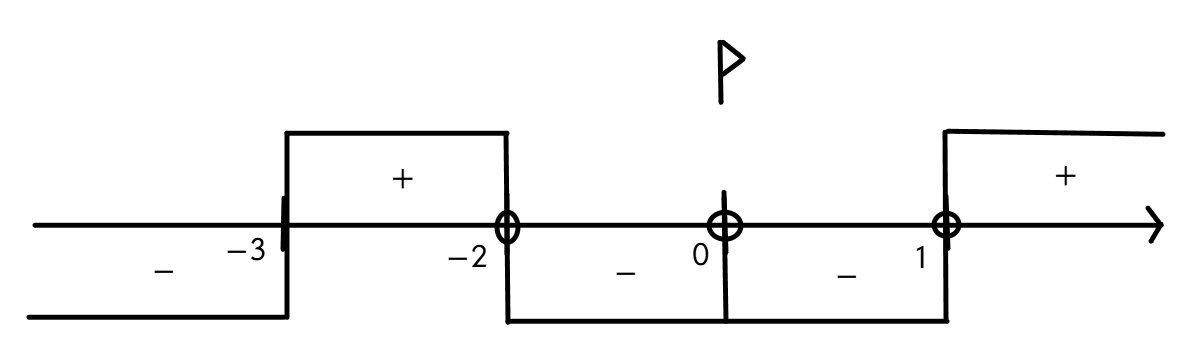
\includegraphics[scale=0.35]{ner9-38.png}}
\end{figure}\\
